\documentclass[conference]{IEEEtran}
\IEEEoverridecommandlockouts
\usepackage{amsmath,amssymb}
\usepackage{graphicx}
\usepackage{booktabs}
\usepackage{stfloats}
\usepackage{cite}
\usepackage[hidelinks]{hyperref}
\graphicspath{{figures/}}
\renewcommand{\topfraction}{0.9}
\renewcommand{\dbltopfraction}{0.9}
\renewcommand{\textfraction}{0.07}
\renewcommand{\floatpagefraction}{0.85}
\renewcommand{\dblfloatpagefraction}{0.85}

\begin{document}

\title{Statistical Modelling of Packet-Loss Patterns in Computer Networks: Distribution Fitting, Burstiness Testing and Bayesian Estimation}

\author{\IEEEauthorblockN{Shashank Tiwari}
\IEEEauthorblockA{VIT Vellore, India\\25BDS0053}
\and
\IEEEauthorblockN{Kyra Panwar}
\IEEEauthorblockA{VIT Vellore, India\\25BBS0095}
\and
\IEEEauthorblockN{Aashman Biyani}
\IEEEauthorblockA{VIT Vellore, India\\25BBS0100}}

\maketitle

\begin{abstract}
Simplest models treat each lost packet as independent of the others which is why most of the times a single number is reported as the loss rate. If this was true, the number of losses in each second would follow a Poisson distribution whereas the gaps between consecutive losses would follow an exponential distribution model. Three networks (wired broadband, campus Wi-Fi and a mobile hotspot) were simulated with a two-state Gilbert-Elliott model, each sending 50 packets per second for 1 hour, which comes to 180{,}000 packets per network. We fitted models for the counts and for the waiting times, tested whether neighbouring packets are independent, and estimated the loss rates with a Bayesian Beta-Binomial model. Independence did not hold on any of the three networks. The variance of the per-second loss count was 1.59, 5.31, 10.17 times the mean, where a Poisson model gives 1, and after a single loss the next packet was 31 to 43 times more likely to be lost. Over 2{,}000 simulated captures, the standard 95\% interval for the loss rate contained the true value in only 40.3\% to 85.7\% of cases. Reducing the sample size by a design effect raised coverage to between 93.3\% and 94.0\%. We then sent 15{,}000 real packets over a mobile hotspot. In both captures with enough losses, independence was rejected again, and a loss made the next one 33 and 51 times more likely.
\end{abstract}

\begin{IEEEkeywords}
Packet loss, Gilbert-Elliott channel, overdispersion, goodness of fit, Bayesian estimation, design effect, Monte Carlo.
\end{IEEEkeywords}

\section{Introduction}
Packet loss is a common issue faced by almost everyone at a certain point in their lives unknowingly. For example, a student attending an online class might have to face audio disruptions and video interruptions. The reason behind this is that packets, which are units of data during transmission, are unable to reach their destination. Applications send packets at a fixed rate and the proportion of the packets that are lost during transmission is known as the packet loss rate. This criterion has an important role in evaluating network performance as it is used to define acceptable level of service quality in service level agreements, helps communication protocols to decide retransmission timers, and also determine the level of error correction needed by a stream.

However, the loss rate cannot depict how the losses are distributed over a period of time. If 10 packets are lost in a scattered manner the decoder is able to hide them and these losses go unnoticed by the user, but a cluster of 10 packet losses will cause an obvious freeze. From our data, the worst single second lost 7 out of 50 on wired, 25 on Wi-Fi, and 40 on mobile connection while most seconds lost none of the packets. Textbooks generally assume that each packet is lost independently with a probability $p$. This would suggest that packet losses occur in a binomial, or almost Poisson, distribution and at the same time the gaps in between consecutive packet losses would be exponential. But on comparing with simulations and subsequent results it is found that these distributions do not actually follow the obtained data once the losses start to cluster.

Our aim was to find out how badly independence fails, which standard tests pick up the failure, and what it does to the interval estimates usually reported for the loss rate. The work is split into two phases. Phase 1 is a simulation study. Because we set the true parameters of each network ourselves, we can compare every estimate and test with the correct answer. In Phase 2 the same code is run on real packets sent over a mobile hotspot.

The paper is organised as follows. Section~II gives some background, Section~III sets out the loss model and the data, Section~IV describes the statistical methods and Section~V reports the results. Section~VI discusses what the results mean and where the study is limited, and Section~VII concludes.

\section{Background}
Modelling bursty errors with a hidden two-state chain goes back to E.~N.~Gilbert, who used it for errors on telephone lines in 1960 \cite{gilbert1960}. In 1963 E.~O.~Elliott extended the model so that errors could occur in either state \cite{elliott1963}. It has also been known for many years that Internet losses are not independent. Measurement studies in the 1990s showed that probe packets sent close together were often lost together \cite{bolot1993}, and that losses in TCP transfers came in correlated episodes \cite{paxson1997}. The timing of loss in multicast traces could be described reasonably well with Markov chains \cite{yajnik1999}. Later studies fitted Gilbert models to voice traffic and related the length of a loss burst to how poor a call sounds \cite{jiang2000,hasslinger2008}.

Most of this earlier work sets out to describe the loss process. Our interest is more statistical. We want to know which standard tests detect the dependence, how much data they need before they do, and how far ordinary interval estimates drift from the truth when the dependence is ignored. For the last of these we use the design effect from survey sampling \cite{kish1965}.

\section{Loss Model and Data}
\subsection{The Gilbert-Elliott Channel}
We treat the network as being in one of two hidden states, Good (G) or Bad (B). We cannot observe the state itself, only what it does to the packets. Before each packet, the channel switches from Good to Bad with probability $p$ and from Bad back to Good with probability $r$. In the Good state a packet is lost with a small probability $h_G$; in the Bad state the probability $h_B$ is much larger. Over a long run, the flow into the Bad state has to equal the flow out of it. This gives the share of time spent in Bad, and from it the overall loss rate:
\begin{equation}
\pi_B=\frac{p}{p+r},\qquad P(\text{loss})=(1-\pi_B)\,h_G+\pi_B\,h_B .
\label{eq:ge}
\end{equation}
The number of packets spent in a state before leaving it is geometric, with a mean of $1/p$ packets for Good and $1/r$ for Bad. A burst of losses happens whenever the channel drops into the Bad state for a few packets.

\subsection{Simulated Networks}
Table~\ref{tab:params} summarizes the parameters for the three networks, namely, wired, Wi-Fi and mobile connections with low, medium and high loss respectively. Close to the rate of a voice call, every network sends 50 packets per second. The simulation lasts for 3600 seconds and produces a total of 180,000 packets per network. Rather than going packet by packet, we take each Good spell and Bad spell straight from the geometric distribution and lay them end to end. All the random numbers were taken from seed 2026, so anybody who reruns the simulation will obtain the exact same numbers.

\begin{table}[!t]
\caption{Scenario Parameters and the True Loss Rate They Imply}
\label{tab:params}
\centering
\footnotesize
\setlength{\tabcolsep}{3.2pt}
\begin{tabular}{lccccccc}
\toprule
Network & $p$ & $r$ & $h_G$ & $h_B$ & $\pi_B$ & Bad spell & True loss \\
\midrule
Wired & 0.0005 & 0.3 & 0.002 & 0.5 & 0.17\% & 3.3 & 0.283\% \\
Wi-Fi & 0.002 & 0.15 & 0.004 & 0.6 & 1.32\% & 6.7 & 1.184\% \\
Mobile & 0.004 & 0.08 & 0.006 & 0.7 & 4.76\% & 12.5 & 3.905\% \\
\bottomrule
\end{tabular}
\\[2pt]
\raggedright\scriptsize Bad spell is the average stay in the Bad state, $1/r$ packets. True loss comes from (\ref{eq:ge}).
\end{table}

\subsection{Real Measurements}
For Phase 2 we wrote a probe that sends 50 numbered ICMP echo requests per second, the same rate as the simulation, and records which replies come back. A packet counts as lost when no reply arrives within 2~s, so this is round-trip loss. The laptop was connected to a mobile phone hotspot on 29 and 30 October 2026. Two captures of 120~s were sent to the hotspot's gateway and two of 30~s to the public address 1.1.1.1 through the same hotspot, giving 15{,}000 packets in all. Each capture is a 0/1 sequence of delivered and lost packets, so every method below runs on it unchanged.

\section{Methodology}
\subsection{Fitting the Distributions}
For the per-window loss counts $x_1,\dots,x_n$, the first model we fit is the Poisson distribution, whose maximum-likelihood estimate is simply the mean count, $\hat\lambda=\bar x$. The natural alternative is the Negative Binomial:
\begin{align}
P(X=k)&=\binom{k+r_{\!NB}-1}{k}q^{r_{\!NB}}(1-q)^k,\\
\operatorname{Var}(X)&=\mu+\mu^2/r_{\!NB} .
\end{align}
The Negative Binomial can be thought of as a Poisson whose rate changes over time, which is what a network moving between good and bad periods produces. The extra term $\mu^2/r_{\!NB}$ lets the variance exceed the mean, something the Poisson cannot do.

For the gaps between losses we begin with the exponential distribution and compare it with a mixture of two exponentials known as the two-phase hyperexponential:
\begin{equation}
f(t)=w\lambda_1e^{-\lambda_1t}+(1-w)\lambda_2e^{-\lambda_2t}.
\end{equation}
Short gaps, with the fast rate $\lambda_1$, occur within a burst. Long gaps, with the slow rate $\lambda_2$, occur between bursts. We never know which type a particular gap is, so we fit the mixture with the Expectation-Maximisation (EM) algorithm \cite{dempster1977}. In each iteration the E-step works out the probability that each gap is a short one, and the M-step updates $w$, $\lambda_1$ and $\lambda_2$ with these probabilities as weights. Models are compared with the Akaike Information Criterion, $\text{AIC}=2k-2\ln L$ \cite{akaike1974}, where a lower value means a better model.

\subsection{Goodness of Fit}
We evaluate the goodness of fit by comparing the observed and expected number of seconds with $k$ losses under each model using the Pearson statistic $\chi^2=\sum_i (O_i-E_i)^2/E_i$, with tail bins merged until every expected count is at least 5. We also check the Poisson assumption by using the index-of-dispersion test. The test statistic is $(n-1)s^2/\bar x$ and follows a $\chi^2_{n-1}$ distribution. A variance which is greater than the mean indicates overdispersion and produces a large statistic value.

For the gaps between losses, the goodness of fit is assessed using the Kolmogorov-Smirnov (KS) distance test $D=\sup_t|F_n(t)-F(t)|$. Here the rate is estimated from the same data, which leaves the textbook p-value too large \cite{lilliefors1969}. Parametric bootstrap is used to get the p-value instead \cite{efron1993}. This procedure is conducted 2,000 times for the exponential and 500 times for the mixture models.

\subsection{Testing Independence}
A run is a sequence of same outcomes. For example, 0\,0\,1\,1\,0\,0\,0 has 3 runs. The Wald-Wolfowitz runs test \cite{wald1940} counts the number of runs $R$. With $n_1$ losses and $n_0$ deliveries, independence gives
\begin{equation}
E[R]=\frac{2n_1n_0}{n}+1,\quad \operatorname{Var}(R)=\frac{2n_1n_0(2n_1n_0-n)}{n^2(n-1)} .
\end{equation}
When losses tend to occur together, the sequence switches between lost and delivered less often than it would by chance, and $R$ ends up smaller than expected.

The Markov-chain test asks the question more directly: does the outcome for one packet depend on the packet before it? Under $H_1$ there are two loss probabilities, $a=P(L\mid N)$ after a delivered packet and $b=P(L\mid L)$ after a lost one. Writing $n_{xy}$ for the number of times outcome $x$ is followed by outcome $y$,
\begin{equation}
\hat a=\frac{n_{NL}}{n_{NN}+n_{NL}},\qquad \hat b=\frac{n_{LL}}{n_{LN}+n_{LL}},
\end{equation}
\begin{equation}
G^2=2(\ln L_1-\ln L_0).
\end{equation}
By Wilks' theorem \cite{wilks1938}, $G^2$ is approximately $\chi^2_1$ when $H_0$ holds. The ratio $b/a$ measures how much a loss raises the chance of the next loss, and $1/(1-b)$ gives the mean burst length.

The networks are compared with the Kruskal-Wallis test \cite{kruskal1952}, pairwise Mann-Whitney tests \cite{mann1947} with a Bonferroni correction, and a chi-square test of homogeneity on total lost and delivered packets. All tests use $\alpha=0.05$.

\subsection{Bayesian Estimation}
We calculate the loss rate in the Bayesian manner \cite{gelman2013}. The prior used is flat, specifically $\text{Beta}(1,1)$, and this assumes that all possible loss rates between 0 and 1 are equally likely prior to any data being observed. Once $k$ losses have been observed among $n$ packets, the posterior distribution becomes $\text{Beta}(1+k,\,1+n-k)$. We give the mean of the posterior together with its 95\% credible interval. The burst parameters are treated the same way, with $a\sim\text{Beta}(1+n_{NL},1+n_{NN})$ and $b\sim\text{Beta}(1+n_{LL},1+n_{LN})$, and these give credible intervals for $b/a$ and for the burst length. To check the independent model, we use it to predict how frequently a window should contain at least five losses and then compare that frequency with the actual frequency at which it occurs.

\subsection{Design Effect}
The variance of a sum shows why bursts cause problems for interval estimates:
\begin{equation}
\operatorname{Var}\Big(\sum_i X_i\Big)=\sum_i\operatorname{Var}(X_i)+2\sum_{i<j}\operatorname{Cov}(X_i,X_j).
\end{equation}
In the case of independent packets each covariance term is zero; within a burst, however, adjacent packets tend to have the same result, the covariances are positive and so the actual variance is greater. The standard interval fails to take this into account and therefore ends up being too narrow.

To correct for it, we divide each trace into blocks of $m=500$ packets (10~s):
\begin{equation}
\text{deff}=\frac{s^2_{\text{block}}}{m\,\hat p(1-\hat p)},\qquad n_{\text{eff}}=\frac{n}{\text{deff}},
\end{equation}
where deff is not allowed to fall below 1. You can interpret $n_{\text{eff}}$ as being equal to the number of independent packets that carry the same information as our correlated ones. The adjusted posterior uses these effective counts, $\text{Beta}(1+k/\text{deff},\,1+(n-k)/\text{deff})$.

\subsection{Monte Carlo Checks}
We are unable to answer two of our questions on the basis of a single trace and therefore answer them by repeating the experiment a number of times. The first is power, the probability that each test notices the bursts, for capture lengths between 15~s and 600~s. The second is coverage: how often a 95\% interval actually includes the true loss rate in 10-minute captures. Each uses 2{,}000 repetitions, so the standard error of each proportion is approximately 0.011. For a real capture the true loss rate is unknown, so we fit a two-state chain with its own $\hat a$ and $\hat b$ and repeat the same checks on it.

\section{Results}

\begin{figure*}[!t]
\centering
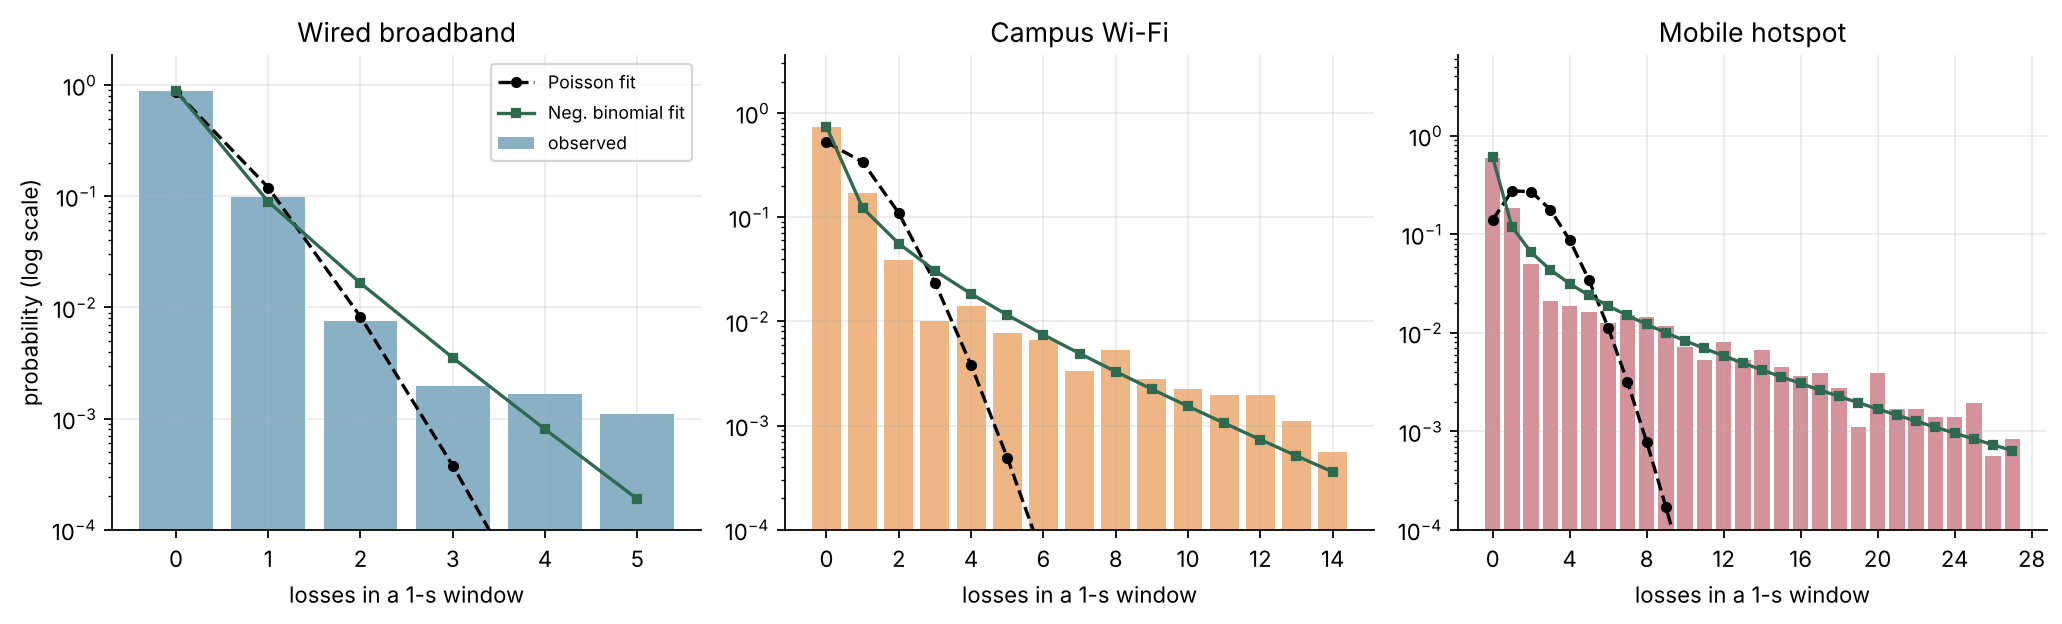
\includegraphics[width=0.86\textwidth]{fig2_count_distribution_fits.png}
\caption{Probability of $k$ losses in one second, on a log scale. The Poisson fit (dashed) falls well below the observed tail, while the Negative Binomial (green) stays close to it.}
\label{fig:counts}
\end{figure*}

\subsection{Loss Counts}
None of the three networks fits the Poisson model, and Table~\ref{tab:sim} shows why. The observed variance is 1.59, 5.31, 10.17 times the mean, and the dispersion test gives $p<10^{-10}$ in each case. The Negative Binomial fits much better and has a lower AIC on all three networks. Most of the difference lies in the tail. For Wi-Fi, the Poisson model expects about 1.98 seconds with 5 or more losses in an hour. The trace contains 131, and the Negative Binomial expects 124.2 (Fig.~\ref{fig:counts}).

\begin{table*}[!t]
\caption{Phase 1 Results for the Three Simulated Networks}
\label{tab:sim}
\centering
\footnotesize
\setlength{\tabcolsep}{4.2pt}
\begin{tabular}{lcccccccccccc}
\toprule
Network & Loss rate & D & AIC Pois. & AIC NB & KS exp. $p$ & Runs $z$ & $P(L|N)$ & $P(L|L)$ & $b/a$ & deff & Naive cov. & Adj. cov. \\
\midrule
Wired & 0.276\% & 1.59 & 3{,}143 & 2{,}992 & $<0.0005$ & -43.5 & 0.25\% & 10.5\% & 43 & 1.52 & 85.7\% & 93.3\% \\
Wi-Fi & 1.293\% & 5.31 & 10{,}607 & 7{,}186 & $<0.0005$ & -146.7 & 0.85\% & 35.4\% & 42 & 6.43 & 60.9\% & 94.0\% \\
Mobile & 3.938\% & 10.17 & 25{,}042 & 11{,}700 & $<0.0005$ & -228.2 & 1.82\% & 55.6\% & 31 & 12.14 & 40.3\% & 94.0\% \\
\bottomrule
\end{tabular}
\\[2pt]
\raggedright\scriptsize Loss rate is the posterior mean. D is the variance of the per-second count divided by its mean. $b/a$ is the posterior median. Coverage is from 2{,}000 simulated 10-minute captures. Every dispersion, runs and Markov test gives $p<10^{-10}$.
\end{table*}

\subsection{Gaps Between Losses}
The exponential model is rejected as well, with the bootstrap KS test failing it on every network. On a log scale an exponential survival curve is a straight line, and the observed curves are not straight. They fall steeply at first, because many of the gaps are very short, and then level off. The mean gap in the fast phase of the mixture is 29 to 33~ms, one to two packets, which matches gaps inside a burst. The slow phase has a mean of 2.1 to 8.6~s and matches the quiet periods between bursts (Fig.~\ref{fig:gaps}).

\begin{figure*}[!t]
\centering
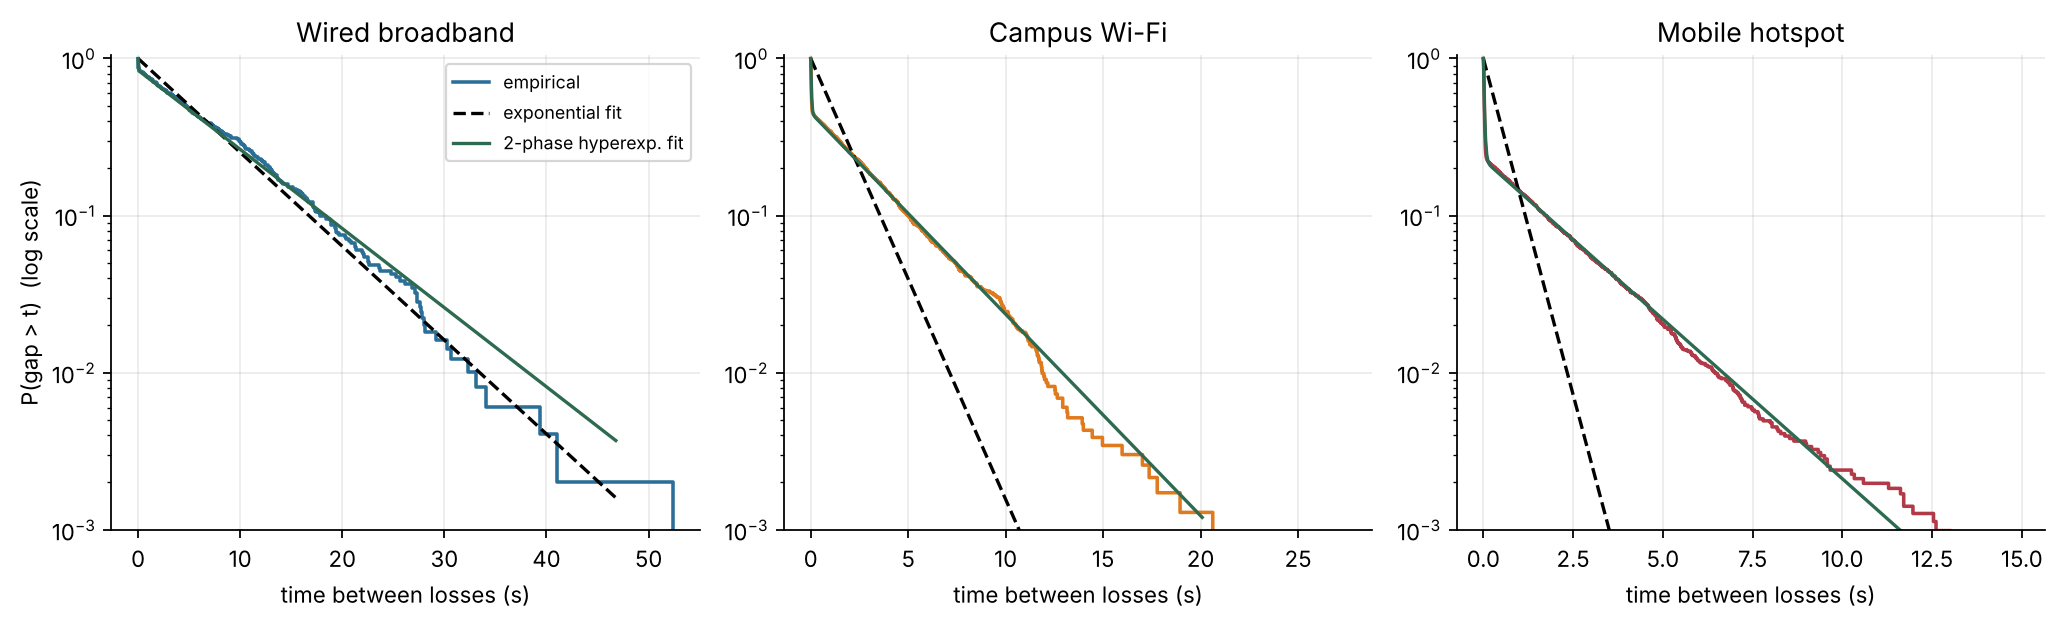
\includegraphics[width=0.86\textwidth]{fig3_gap_survival.png}
\caption{Probability that the gap between two losses is longer than $t$, on a log scale. The exponential fit is a straight line (dashed); the two-phase mixture (green) bends with the data.}
\label{fig:gaps}
\end{figure*}

\subsection{Do Losses Depend on Each Other?}
They clearly do. Both independence tests reject $H_0$ with $p<10^{-10}$ on every network. For Wi-Fi we count 3{,}005 runs, against about 4{,}593 expected under independence. On Wi-Fi a packet is lost 0.85\% of the time when the packet before it was delivered, but 35.4\% of the time when the packet before it was lost. The posterior medians of $b/a$ are 43, 42, 31 for Wired, Wi-Fi and Mobile (Fig.~\ref{fig:markov}). The average bursts are short, at 1.12, 1.55, 2.25 packets, but they happen far more often than they would by chance.

\subsection{Comparing the Networks}
The three networks differ clearly, as expected from how they were set up. The Kruskal-Wallis statistic is $H=937.3$, the $\chi^2$ homogeneity statistic is 7{,}143.0 on 2 degrees of freedom, and even the largest Bonferroni-corrected pairwise p-value is $<10^{-10}$. With only 10~s of Campus Wi-Fi traffic the estimate is 3.78\% [2.30\%, 5.62\%], a wide interval. After 3{,}600~s it has narrowed to 1.29\% [1.24\%, 1.35\%].

The predictive check shows how poorly the independent model handles seconds with many losses. For Wi-Fi it puts the probability of a second with at least 5 losses at 0.00047. In the trace such seconds make up 0.036 of the total, about 77 times as often as predicted.

\begin{figure}[!t]
\centering
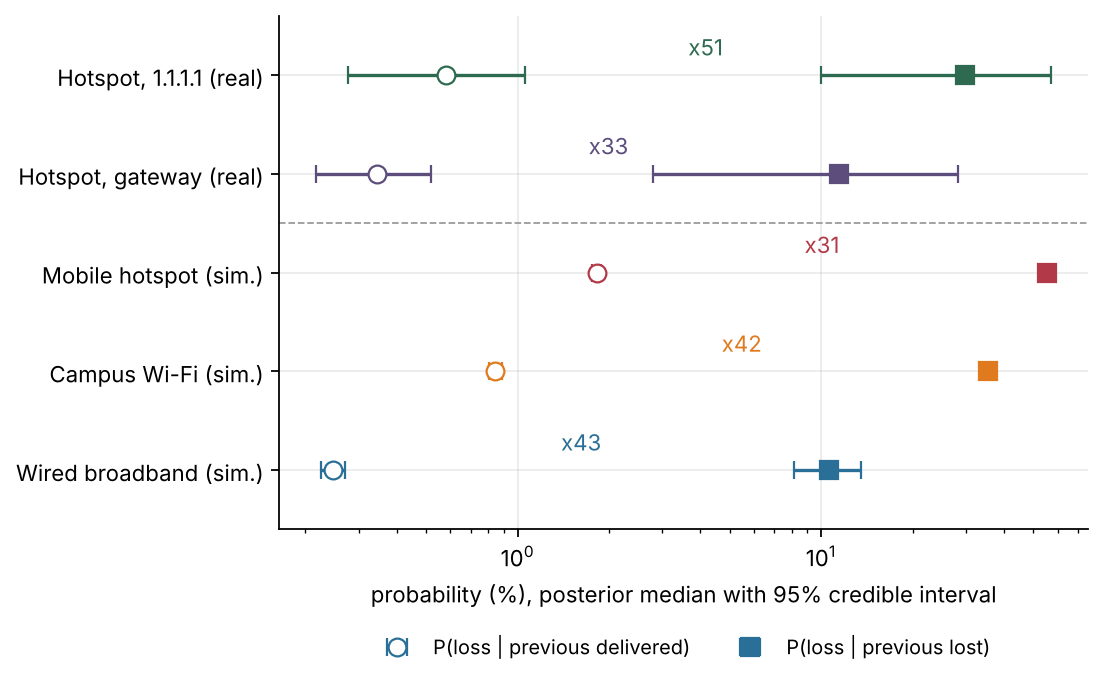
\includegraphics[width=\columnwidth]{fig_markov_sim_real.png}
\caption{Posterior medians and 95\% credible intervals for $P(L\mid N)$ (open) and $P(L\mid L)$ (filled), for the simulated networks and the two real hotspot captures with enough losses.}
\label{fig:markov}
\end{figure}

\subsection{How Often Do the Intervals Work?}
For us this is the key result. Across 2{,}000 simulated 10-minute captures, the naive 95\% interval included the true loss rate in only 85.7\%, 60.9\%, 40.3\% of cases (Fig.~\ref{fig:coverage}). On the burstiest network it missed the true value more often than it caught it. The design effects are 1.52, 6.43 and 12.14. For Wi-Fi, this means our 180{,}000 packets hold roughly the same information as 28{,}000 independent packets would. With these smaller effective sample sizes, coverage returns to 93.3\%, 94.0\%, 94.0\%, close to the intended 95\%. The full Wi-Fi trace is a good example. Its true loss rate is 1.184\%. The naive interval of [1.241\%, 1.345\%] lies entirely above this value, while the adjusted interval of [1.167\%, 1.431\%] contains it.

\begin{figure}[!t]
\centering
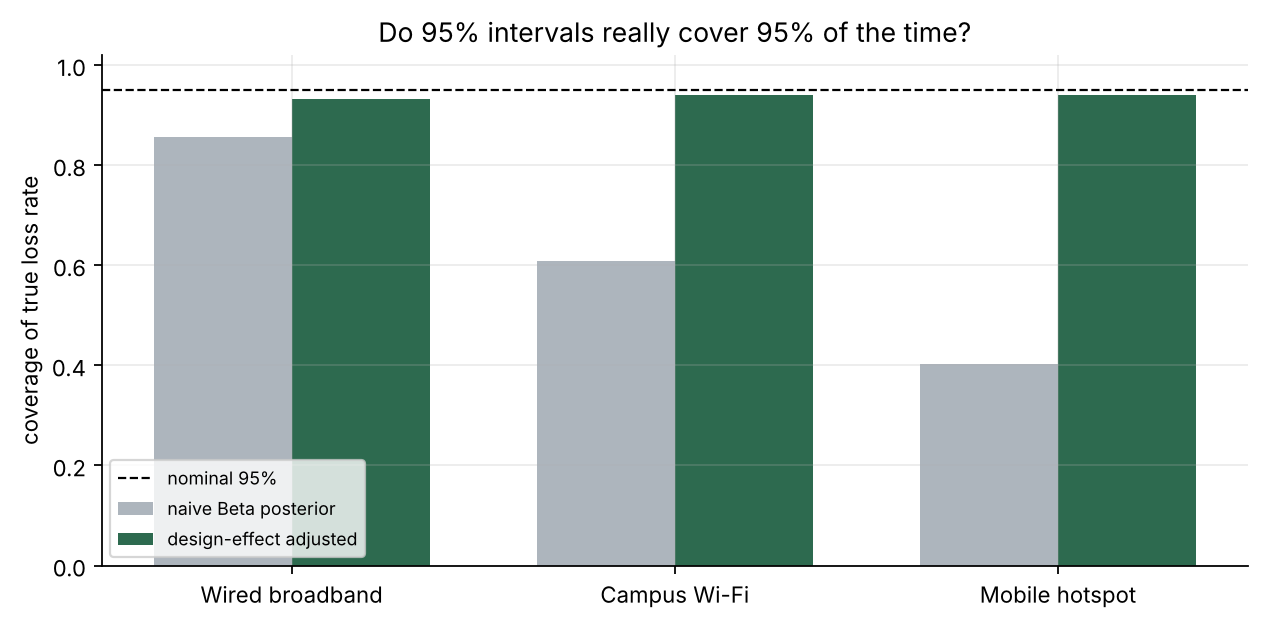
\includegraphics[width=0.9\columnwidth]{fig7_interval_coverage.png}
\caption{Share of nominal 95\% intervals that contain the true loss rate, before and after the design-effect correction.}
\label{fig:coverage}
\end{figure}

\subsection{How Long Should a Capture Be?}
With the runs test, the mobile network needs only 15~s to reach a power of 0.8 and Wi-Fi 30~s. Wired needs 300~s, since its bursts are infrequent and short. At 600~s every test has a power of at least 0.97 on every network.

\subsection{Real Hotspot Captures}
Table~\ref{tab:real} lists the four real captures. Two of them lost too few packets to test. The first gateway capture lost 22 of 6{,}000 packets and the second lost none, so a hotspot link can be clean on one day and lossy on another. Through to 1.1.1.1 the round-trip time was far higher, with a median of 50 to 131~ms against 4 to 7~ms to the gateway.

The two captures with at least 10 losses tell the same story as the simulation. On the gateway capture a packet was lost 0.34\% of the time after a delivery but 9.1\% of the time after a loss, and on the 1.1.1.1 capture 0.54\% against 27.3\%. The posterior medians of $b/a$ are 33 and 51, inside or above the 31 to 43 range of the simulated networks (Fig.~\ref{fig:markov}). The Markov test rejects independence on both, with $p=0.002$ and $p=3\times10^{-5}$, and so does the dispersion test. The exponential model for the gaps is rejected on the 1.1.1.1 capture ($p=0.001$), where the fast phase of the mixture has a mean gap of 34~ms, close to the 29 to 33~ms found in the simulation.

Fitting a two-state chain to each capture and repeating it 2{,}000 times shows the same weakness in the naive interval. For 10-minute captures it would cover the true rate in 93.1\% and 86.8\% of cases, and the adjusted interval in 94.7\% and 94.4\%. The runs test would have a power of 0.83 at 120~s on the gateway link and 0.999 at 600~s, which again supports recording for ten minutes.

\begin{table}[!t]
\caption{Real Captures over a Mobile Hotspot}
\label{tab:real}
\centering
\footnotesize
\setlength{\tabcolsep}{2.6pt}
\begin{tabular}{lcccccc}
\toprule
Target & Length & Lost & Loss rate [95\% CrI] & RTT & $b/a$ & Markov $p$ \\
\midrule
Gateway & 120 s & 22 & 0.38\% [0.24, 0.55] & 6.8 ms & 33 & 0.002 \\
Gateway & 120 s & 0 & 0.02\% [0.00, 0.06] & 3.7 ms & n/a & n/a \\
1.1.1.1 & 30 s & 1 & 0.13\% [0.02, 0.37] & 50 ms & n/a & n/a \\
1.1.1.1 & 30 s & 11 & 0.80\% [0.41, 1.31] & 131 ms & 51 & $3\times10^{-5}$ \\
\bottomrule
\end{tabular}
\\[2pt]
\raggedright\scriptsize Loss rate is the posterior mean. RTT is the median round-trip time. Tests need at least 10 losses.
\end{table}

\section{Discussion and Limitations}
It takes surprisingly little for independence to fail. A Bad spell of only a few packets is enough to break every model built on that assumption, and the loss rate alone gives no hint of it. Mobile loses roughly 14 times as many packets as Wired, yet on both networks a loss makes another loss tens of times more likely. The real hotspot behaved the same way, even at a loss rate below 1\%. Burstiness is a separate property of a link and has to be measured separately.

The coverage results show the problem is bigger than picking the right model. A naive interval counts every packet as a new and independent piece of evidence. When packets within a burst share the same outcome, there is much less independent evidence than the packet count suggests, and the interval turns out too narrow. The design-effect correction is simple, needs only block counts, and brings coverage close to 95\% on all three networks.

Our conclusions are limited by certain factors. The simulated data comes from the same model that motivated the study. The real captures are short, come from one hotspot and one laptop, and only two of them had enough losses to test. With 11 and 22 losses the credible intervals for $b/a$ are wide, and the large-sample approximation behind the runs test is rough, so we rely mainly on the Markov test. Loss is measured on the round trip, and ICMP replies may be treated differently from other traffic. The design effect also needs several 10-s blocks, so it says little about a 30-s capture.

\section{Conclusion and Future Work}
We tested whether packet losses behave independently, and found that they do not. On three simulated networks the per-second loss counts were 1.59, 5.31, 10.17 times more spread out than a Poisson model allows, and each loss made the next one 31 to 43 times more likely. The standard 95\% interval for the loss rate was right in only 40.3\% to 85.7\% of cases, and dividing the sample size by the design effect raised this to between 93.3\% and 94.0\%. Real packets sent over a mobile hotspot showed the same dependence, with a loss making the next one 33 and 51 times more likely.

Next we will record captures of at least ten minutes on wired, Wi-Fi and mobile links at peak and off-peak hours, estimate the Gilbert-Elliott parameters from them with the Baum-Welch algorithm \cite{baum1970}, and use the Phase 1 results as priors in a hierarchical Bayesian model. All results were produced by one Python pipeline built on NumPy \cite{numpy2020}, SciPy \cite{scipy2020} and Matplotlib \cite{matplotlib2007}, run with seed 2026.

\begin{thebibliography}{99}
\bibitem{gilbert1960} E. N. Gilbert, ``Capacity of a burst-noise channel,'' \emph{Bell Syst. Tech. J.}, vol. 39, no. 5, pp. 1253--1265, 1960.
\bibitem{elliott1963} E. O. Elliott, ``Estimates of error rates for codes on burst-noise channels,'' \emph{Bell Syst. Tech. J.}, vol. 42, no. 5, pp. 1977--1997, 1963.
\bibitem{bolot1993} J.-C. Bolot, ``End-to-end packet delay and loss behavior in the Internet,'' in \emph{Proc. ACM SIGCOMM}, 1993, pp. 289--298.
\bibitem{paxson1997} V. Paxson, ``End-to-end Internet packet dynamics,'' in \emph{Proc. ACM SIGCOMM}, 1997, pp. 139--152.
\bibitem{yajnik1999} M. Yajnik, S. Moon, J. Kurose, and D. Towsley, ``Measurement and modelling of the temporal dependence in packet loss,'' in \emph{Proc. IEEE INFOCOM}, 1999, pp. 345--352.
\bibitem{jiang2000} W. Jiang and H. Schulzrinne, ``Modeling of packet loss and delay and their effect on real-time multimedia service quality,'' in \emph{Proc. NOSSDAV}, 2000.
\bibitem{hasslinger2008} G. Hasslinger and O. Hohlfeld, ``The Gilbert-Elliott model for packet loss in real time services on the Internet,'' in \emph{Proc. 14th GI/ITG Conf. MMB}, 2008, pp. 269--286.
\bibitem{kish1965} L. Kish, \emph{Survey Sampling}. New York: Wiley, 1965.
\bibitem{dempster1977} A. P. Dempster, N. M. Laird, and D. B. Rubin, ``Maximum likelihood from incomplete data via the EM algorithm,'' \emph{J. Roy. Statist. Soc. B}, vol. 39, no. 1, pp. 1--38, 1977.
\bibitem{akaike1974} H. Akaike, ``A new look at the statistical model identification,'' \emph{IEEE Trans. Autom. Control}, vol. 19, no. 6, pp. 716--723, 1974.
\bibitem{lilliefors1969} H. W. Lilliefors, ``On the Kolmogorov-Smirnov test for the exponential distribution with mean unknown,'' \emph{J. Amer. Statist. Assoc.}, vol. 64, pp. 387--389, 1969.
\bibitem{efron1993} B. Efron and R. J. Tibshirani, \emph{An Introduction to the Bootstrap}. New York: Chapman \& Hall, 1993.
\bibitem{wald1940} A. Wald and J. Wolfowitz, ``On a test whether two samples are from the same population,'' \emph{Ann. Math. Statist.}, vol. 11, no. 2, pp. 147--162, 1940.
\bibitem{wilks1938} S. S. Wilks, ``The large-sample distribution of the likelihood ratio for testing composite hypotheses,'' \emph{Ann. Math. Statist.}, vol. 9, no. 1, pp. 60--62, 1938.
\bibitem{kruskal1952} W. H. Kruskal and W. A. Wallis, ``Use of ranks in one-criterion variance analysis,'' \emph{J. Amer. Statist. Assoc.}, vol. 47, pp. 583--621, 1952.
\bibitem{mann1947} H. B. Mann and D. R. Whitney, ``On a test of whether one of two random variables is stochastically larger than the other,'' \emph{Ann. Math. Statist.}, vol. 18, no. 1, pp. 50--60, 1947.
\bibitem{gelman2013} A. Gelman, J. B. Carlin, H. S. Stern, D. B. Dunson, A. Vehtari, and D. B. Rubin, \emph{Bayesian Data Analysis}, 3rd ed. Boca Raton, FL: CRC Press, 2013.
\bibitem{baum1970} L. E. Baum, T. Petrie, G. Soules, and N. Weiss, ``A maximization technique occurring in the statistical analysis of probabilistic functions of Markov chains,'' \emph{Ann. Math. Statist.}, vol. 41, no. 1, pp. 164--171, 1970.
\bibitem{numpy2020} C. R. Harris \emph{et al.}, ``Array programming with NumPy,'' \emph{Nature}, vol. 585, pp. 357--362, 2020.
\bibitem{scipy2020} P. Virtanen \emph{et al.}, ``SciPy 1.0: Fundamental algorithms for scientific computing in Python,'' \emph{Nature Methods}, vol. 17, pp. 261--272, 2020.
\bibitem{matplotlib2007} J. D. Hunter, ``Matplotlib: A 2D graphics environment,'' \emph{Comput. Sci. Eng.}, vol. 9, no. 3, pp. 90--95, 2007.
\end{thebibliography}

\end{document}
